\chapter{Additional Context}
\label{chapterlabel3}

In this chapter we provide a review of the case studies that are investigated in this project and offer a justification for why they were each selected. For each humanitarian case study, we provide contextual information regarding the associated humanitarian crisis and the mapping efforts that ensued. We also provide a summary of the way that spatial data is stored in OSM, to give context to the analysis and interpretation of results that will be provided in subsequent chapters.


\section{Case studies}

The scope of this work is limited to four humanitarian mapping case studies and one reference case study. We selected humanitarian case studies that consisted of mapping efforts in response to a humanitarian need, were constrained to subnational geographic areas, drove a sufficient volume of mapping activity on OSM (as defined by volume of unique contributors and volume of edits over time), and were sufficiently documented on pages such as the OSM Wiki\footnote{\url{https://wiki.openstreetmap.org/wiki/Main_Page}}, HOT Projects page\footnote{\url{https://www.hotosm.org/projects/}}, or HOT Tasking Manager\footnote{\url{https://tasks.hotosm.org/}}. We have also selected case studies that capture practices of humanitarian mapping at various stages in the history of the humantiarian OSM community. However, we have not selected any cases that have occurred within the last five years, to allow for the study of maintenance practices in the years following a mapping activation.  

Following from the above criteria, we focus on humanitarian mapping activities in 1) Port au Prince, Haiti, following the 2010 earthquake, 2) Tacloban, Philippines, following the 2015 typhoon, 3) Bangui, Central African Republic, following 2013 rebellions, and 4) Kathmandu, Nepal, following the 2015 earthquake. In addition to these four humanitarian case studies, we have also selected a 'reference' case study as a contrasting example of mapping activities in a region with a highly active and matured OSM community. Following \textcite{anderson_crowd_2018}, we select Heidelberg, Germany as our reference case. 

Background context for the crises that drove the humanitarian mapping activation are provided in the following subsections.

\subsection{Port au Prince, Haiti}

Haiti experienced a magnitude 7.0 earthquake on January 12, 2010, which caused an estimated 300,000 deaths, and widespread building damage and population displacement \parencite{desroches_overview_2011}. The effects of the earthquake were further exacerbated by an outbreak of cholera in October 2010 that spread to informal settlements \parencite{noauthor_world_2011}. It is estimated that this event has caused USD \$8.1bn damage \parencite{cavallo_estimating_2010}. Humanitarian mapping efforts in Haiti following this earthquake have been well researched and discussed in past academic literature \parencite{zook_volunteered_2010, soden_crowdsourced_2014, palen_success_2015, meier_crisis_2012}. This disaster has been described as a 'catalyzing event' for many digitally-focused volunteer communities \parencite[p. 314]{soden_crowdsourced_2014}. Mapping efforts around this event also led to the formalization of the Humanitarian OpenStreetMap Team (HOT), the process of which is described in further detail by \textcite{soden_crowdsourced_2014}. Throughout their post-disaster efforts to raise awareness of the value of OSM and mobilize a community of mappers, one of HOT's primary goals was to 'embed' OSM within the local community and further local ownership of this data. This effort was intended to allow for the long-term use of OSM data beyond this humanitarian response \parencite{soden_crowdsourced_2014}.

\subsection{Tacloban, Philippines}

The Philippines was greatly impacted by a tropical cyclone, Typhoon Haiyan (or Typhoon Yolanda), on November 8, 2013. This typhoon is said to be one of the strongest ever recorded \parencite{lum_typhoon_2014}. USAID estimates that this disaster has caused over 6,000 deaths and the destruction or damage of over 1 million homes \parencite{noauthor_typhoon_2014}. The city of Tacloban was one of the areas that faced greatest impact and was thus where much relief effort was focused \parencite{lum_typhoon_2014}. Following this crisis, mapping efforts in OSM were coordinated by HOT, with high-volume, remote mapping efforts organized by the newly developed Tasking Manager \parencite{noauthor_wikiproject_2018}. \textcite{palen_success_2015} note that the mapping efforts in the Philippines were facilitated by these new tools for technical collaboration, which incorporated lessons learned from previous humanitarian mapping efforts, such as in Haiti. Details from the OSM Wiki page indicate that most mapping efforts were focused on buildings, roads, and infrastructure damage \parencite{noauthor_wikiproject_2018}. 

\subsection{Bangui, Central African Republic}

Violence and instability in CAR mounted in March 2013 when the Seleka rebel group seized the capital city, Bangui \parencite{noauthor_violence_2020}. This event launched a humanitarian mapping activation that aimed to provide baseline geospatial data for the country \parencite{noauthor_wikiproject_2020-1}. Mapping the country's road network was a priority of this activation, as well as mapping affected cities and towns, as idenfitied by local humanitarian stakeholders \parencite{noauthor_wikiproject_2020-1}. UNICEF data for health facilities, water points, and schools was also imported as part of this activation \parencite{noauthor_wikiproject_2020-1}.

\subsection{Kathmandu, Nepal}

Nepal was hit with a magnitude 7.6 earthquake on April 25th, centered approximated 76 km northwest of Kathmandu, which was followed by over 300 aftershocks of over 4.0 magnitude \parencite{noauthor_nepal_2015}. It is estimated that over 9,000 people died in these disasters and over half a million homes were destroyed or damaged \parencite{noauthor_nepal_2015}. The major earthquake and its aftershocks caused further disasters such as landslides and avalanches, and exacerbated vulnerabilities to flooding in many areas \parencite{noauthor_nepal_2015}. As is described by \textcite{soden_infrastructure_2016} this crisis can be viewed as a turning point in the history of post-disaster mapping in the OSM community. Whereas in the Haiti case where HOT needed to conduct notable outreach to spread awareness of the applicability of OSM data, interviews with GIS practitioners in the field found that up-to-date OSM data came to be an 'expected resource' in Nepal \parencite[p. 2801]{soden_infrastructure_2016}


\section{Data description}

The data for this analysis was collected from OSM history extract files. While OSM is most often consumed as a user-facing map, it primarily functions as a geospatial database. The OSM data model uses nodes, ways, and relations to represent the geometry of all geographic entities \parencite{noauthor_elements_2020}. Nodes commonly represent point features, such as shops, healthcare facilities, and bus stops. Ways are ordered collections of nodes, commonly used to represent features such as roads. Closed ways (where the start and end node are the same) are used to represent areal features, such as buildings. Relations are the least common element, used to represent relationships between multiple data elements. Relations can take many forms, but may, for example, be used describe turn restrictions between road sections \parencite{noauthor_elements_2020}. 

The attributes for all OSM elements are stored using tags, which consist of text key, value pairs. An element can have multiple tags, however each key for a single elements must be unique \parencite{noauthor_tags_2020}. While OSM does not impose any restrictions on the contents of a tag (aside from being a 255-character Unicode string), it is a best-practice within the community to follow established tagging conventions for commonly occurring elements \parencite{noauthor_tags_2020}. For example, the \texttt{highway=residential} tag is used to describe roads that provide access to homes \parencite{noauthor_elements_2020}. The Taginfo website\footnote{\url{https://taginfo.openstreetmap.org/}} allows one to see commonly used tags across the world. Each OSM element also contains metadata such as the timestamp of last edit, version number, and user ID of the contributor \parencite{noauthor_elements_2020}. 

OSM data is commonly downloaded from services such as Geofabrik\footnote{\url{https://www.geofabrik.de/}} or Planet OSM\footnote{\url{https://planet.osm.org/}} in SHP, PBF, or OSM XML format \parencite{mooney_accessing_2011}. An example of the OSM XML format can be found on the relevant OSM Wiki page \parencite{noauthor_osm_2017}. From these services, one can download a copy of the database for the full planet, or from selected continents or countries. This files are usually frequently updated (eg. daily, in the case of Geofabrik) to ensure that new contributions or edits to OSM are reflected in the downloadable data. One can download both current snapshots and full historical OSM data from these services. The historical data provides access to all edits that were ever made in OSM and can allow one to understand various aspects of how the map has matured over time \parencite{corcoran_analysing_2013, mooney_characteristics_2012}. Researchers are able to understand the evolution of individual entities in the map, as each entity has an associated version number that allows one to track all revisions \parencite{noauthor_elements_2020}. 

Analyzing historical OSM data has traditionally been challenging, in part due to the incredibly large file size \parencite{raifer_oshdb_2019, mooney_accessing_2011}. At the time of writing, the full history planet OSM XML file is 140 GB, which is too large for many users or researchers to manage effectively without significant technical expertise. As is surveyed by \textcite{raifer_oshdb_2019}, researchers and practitioners have developed numerous tools and algorithms that allow for simpler processing and querying of this large historical dataset. Examples include the \textit{Is OSM Up-To-Date?} website developed by \textcite{minghini_open_2018}, and the \textit{OSMatrix} website developed by \textcite{roick_technical_2012}. 

The current state-of-the-art in this domain is the recently developed OSHDB framework, which provides a flexible and fast way to perform spatio-temporal analyses on historical OSM data \parencite{raifer_oshdb_2019}. The OSHDB framework allows for the extracted historical OSM data to be stored in any JDBC (Java database connectivity) compliant database system and accessed through an API \parencite{raifer_oshdb_2019}. A custom data model was also developed to allow for more efficient access and parallel processing, as is shown in \ref{fig:oshdb}. Each version of an OSM Entity is grouped by a common ID into a parent OSH Entity. Each OSH Entity has a 'type' that corresponds to one of the OSM data types (nodes, ways, or relations) \parencite{raifer_oshdb_2019}. 

%%%%%%%%%%%%%%%%%%%%%%%%%% DATA MODEL IMAGE 
\begin{figure} % opens the figure environment. the '[H]' forces the image to be Here
    \centering % puts the image in the horizontal centre of the page
    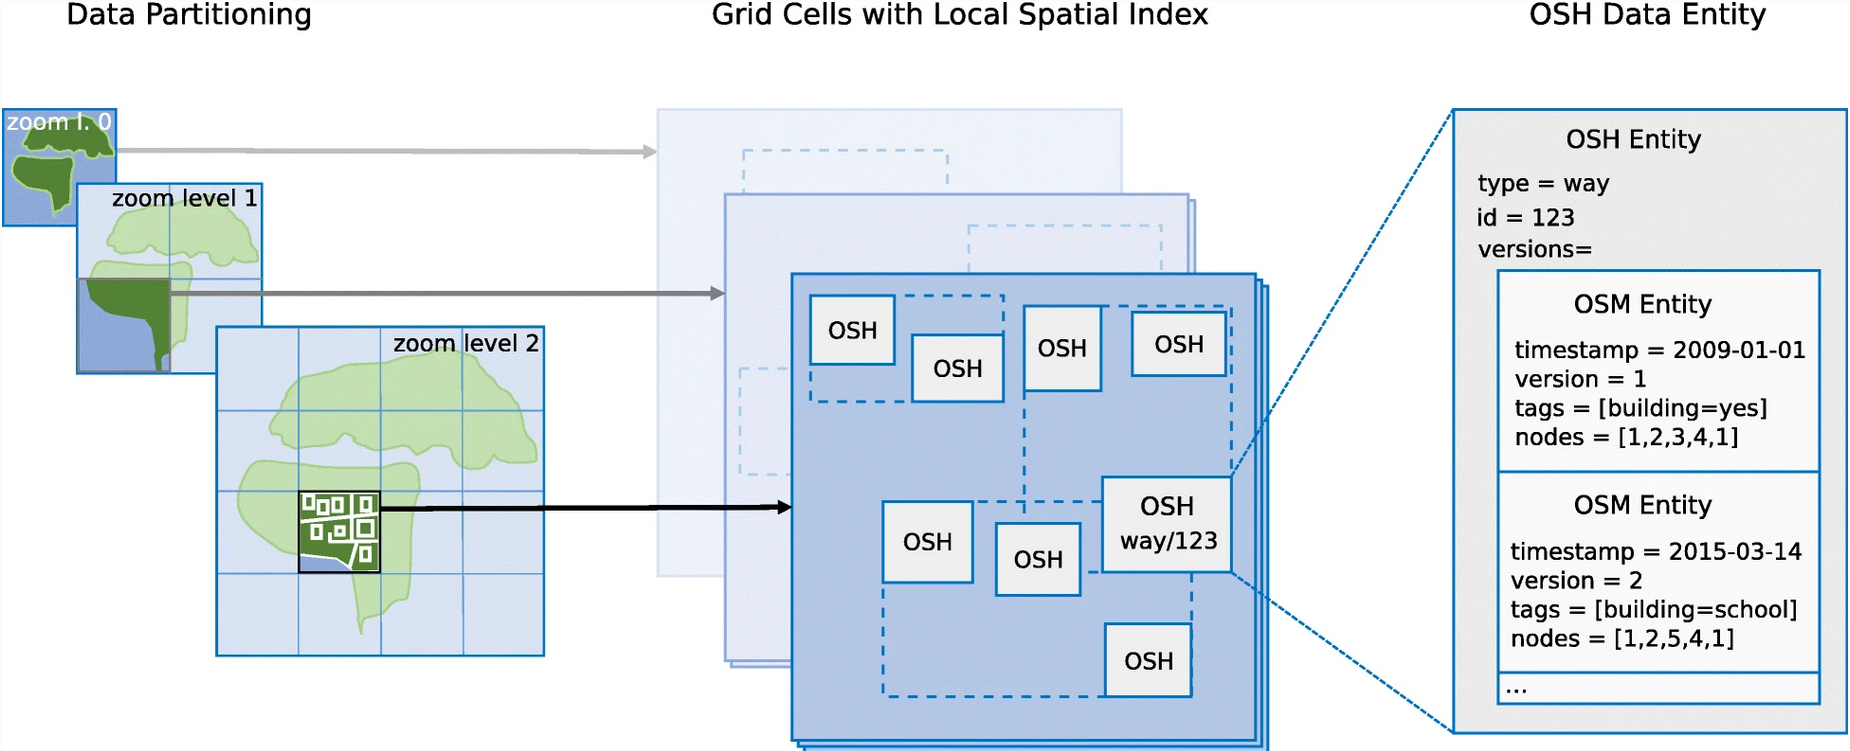
\includegraphics[width = \textwidth]{Images/oshdb.PNG} %this tells latex what graphics to include. 
    \caption{Summary of the OSHDB data model, provided by \textcite{raifer_oshdb_2019}} % this prints the caption below the figure
    \label{fig:oshdb} % this internally labels the figure for future referencing.
\end{figure}
%%%%%%%%%%%%%%%%%%%%%%%%%% 




    


